\section{Příklad 1}
% Jako parametr zadejte skupinu (A-H)
\prvniZadani{E}

\begin{large}
\textbf{Riešenie:} (Metoda postupného zjednodušování obvodu):\\
\end{large}

\textbf{·}
Začneme rezistormi $R_4$ a $R_5$, ktoré sú v paralelnom zapojení.

\begin{center}
$R_{45} = \frac{R_4\cdot{R_5}}{R_4 + R_5} = \frac{340\cdot 575}{340 + 575} = {213,6612} \hspace{0,1cm} \SI{}{\ohm}$\\
\end{center}

\begin{figure}[h!]
    \centering
    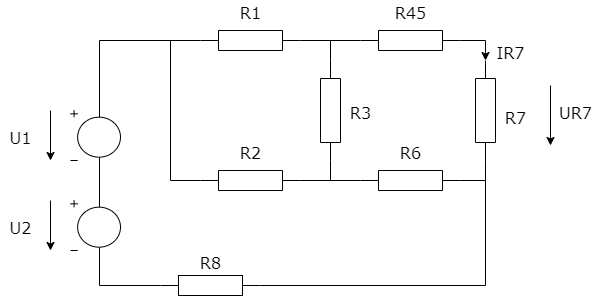
\includegraphics[width=0.75\textwidth]{IEL-Project/pictures/Pr1_1.png}
\end{figure}

\textbf{·}
Ďalej si spracujeme rezistory $R_{45}$ a $R_7$, ktoré sú zapojené sériovo.

\begin{center}
$R_{457} = R_{45} + R_7 = 213,6612 + 255 = 468,6612 \hspace{0,1cm} \SI{}{\ohm}$\\
\end{center}

\begin{figure}[h!]
    \centering
    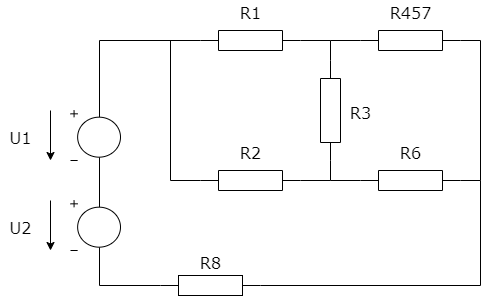
\includegraphics[width=0.6\textwidth]{IEL-Project/pictures/Pr1_2.png}
\end{figure}

\newpage

\textbf{·}
V ďalšom kroku si pomôžeme transfiguráciou trojuholníka na hviezdu.\\

\begin{figure}[h!]
    \centering
    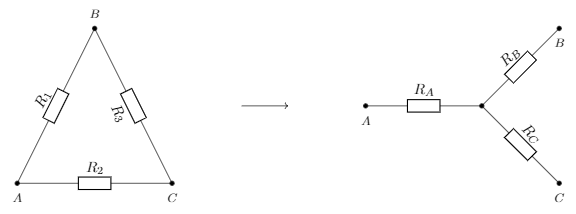
\includegraphics[width=0.75\textwidth]{IEL-Project/pictures/Pr1_3.png}
\end{figure}

\begin{center}
$R_{A}$ = $\frac{R_1 \cdot R_{2}}{R_1 + R_2 + R_3}$ = $\frac{485\cdot660}{485 + 660 + 100} = 257,1084 \hspace{0,1cm} \SI{}{\ohm} $
\end{center}

\begin{center}
$R_{B}$ = $\frac{R_1 \cdot R_{3}}{R_1 + R_2 + R_3}$ = $\frac{485\cdot100}{485 + 660 + 100} = 38,9558 \hspace{0,1cm} \SI{}{\ohm} $
\end{center}

\begin{center}
$R_{C}$ = $\frac{R_2 \cdot R_3}{R_1 + R_2 + R_3}$ = $\frac{660 \cdot 100}{485 + 660 + 100} = 53,012 \hspace{0,1cm} \SI{}{\ohm}$
\end{center}

\begin{figure}[h!]
    \centering
    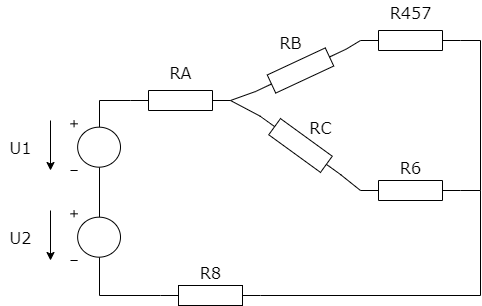
\includegraphics[width=0.6\textwidth]{IEL-Project/pictures/Pr1_4.png}
\end{figure}

\textbf{·}
Z obrázku vidíme, že rezistory $R_B$ a $R_457$ a tiež rezistory $R_C$ a $R_6$ sú v sériovom zapojení, teda môžeme sčítať ich odpory.\\

\begin{center}
$R_{B457}$ = $R_B$ + $R_{457}$ = $ 38,9558 + 468,6612$ = $507,617 \hspace{0,1cm} \SI{}{\ohm}$
\end{center}

\begin{center}
$R_{C6}$ = $R_C$ + $R_6$ = $ 53,012 + 815$ = $868,012 \hspace{0,1cm} \SI{}{\ohm}$
\end{center}

\begin{figure}[h!]
    \centering
    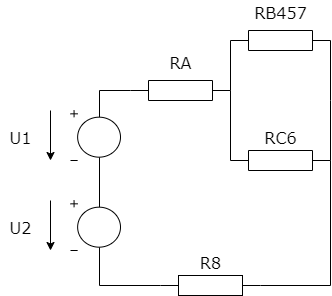
\includegraphics[width=0.5\textwidth]{IEL-Project/pictures/Pr1_5.png}
\end{figure}

\textbf{·}
Z obvodu je zrejmé, že rezistory $R_{B457}$ a $R_{C6}$ sú zapojené paralelne.\\

\begin{center}
$R_{B457C6} = \frac{R_{B457} \cdot R_{C6}}{R_{B457} + R_{C6}} = \frac{507,617 \cdot 868,012}{507,617 + 868,012} = 320,3027 \hspace{0,1cm} \SI{}{\ohm}$
\end{center}

\begin{figure}[h!]
    \centering
    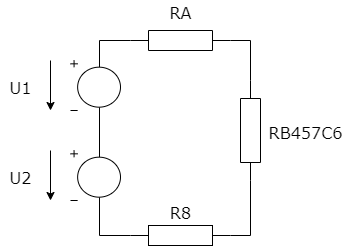
\includegraphics[width=0.5\textwidth]{IEL-Project/pictures/Pr1_6.png}
\end{figure}

\textbf{·}
Nakoniec sčítame odpory zostávajúcich rezistorov, pretože vídíme, že sú zapojené sériovo.\\

\begin{center}
$R_{EKV} = R_{A} + R_{B457C6} + R_{8}  = 257,1084 + 320,3027 + 225 = 802,4111 \hspace{0,1cm} \SI{}{\ohm}$
\end{center}

\begin{figure}[h!]
    \centering
    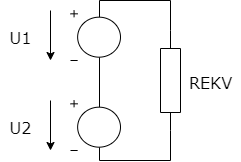
\includegraphics[width=0.35\textwidth]{IEL-Project/pictures/Pr1_7.png}
\end{figure}

\newpage

\textbf{·}
Keďže vieme celkový odpor obvodu, vieme si dopočítať počiatočný prúd. Využijeme na to Ohmov zákon.\\

\begin{center}   
$I = \frac{U_1 + U_2}{R_{EKV}} = \frac{115 + 55}{802,4111} = 0,2119 \hspace{0,1cm} \SI{}{\ampere}$ \\
\end{center}

\textbf{·}
Potrebujeme získať prúd a napätie na rezistore č. 7, to znamená, že budeme obvod spätne „rozkladať“.\\

\begin{figure}[h!]
    \centering
    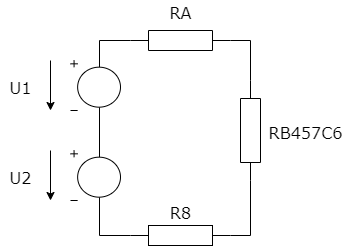
\includegraphics[width=0.5\textwidth]{IEL-Project/pictures/Pr1_6.png}
\end{figure}

\textbf{·}
Rezistory $R_A$, $R_{B457C6}$ a $R_8$ sú zapojené sériovo, tým pádom je jasné, že všetkými rezistormi preteká rovnaký prúd. Napätie na týchto rezistoroch bude ale odlišné, preto si vypočítame napätie $U_{B457C6}$.

\begin{center}
$U_{B457C6} = I\cdot{R_{B457C6}} = 0,2119\cdot{320,3027} = 67,8721  \hspace{0,1cm} \SI{}{\volt}$ 
\end{center}

\textbf{·}
V ďalšom kroku sa vrátime ku zapojení hviezdy, kde vidíme, že pre vypočítanie $U_{R7}$ a $I_{R7}$ potrebujeme vypočítať $U_{R457}$ a $I_{R457}$.\\

\begin{figure}[h!]
    \centering
    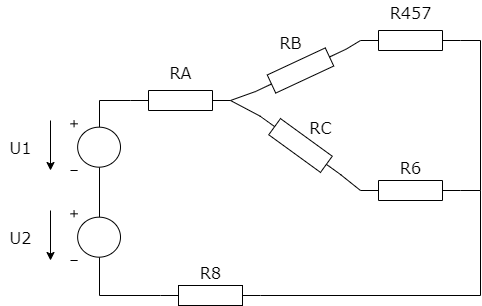
\includegraphics[width=0.6\textwidth]{IEL-Project/pictures/Pr1_4.png}
\end{figure}

\newpage

\begin{center}
$I_{B457} = \frac{U_{B457C6}}{R_{B457}} = \frac{67,8721}{507,617} = 0,1337 \hspace{0,1cm} \SI{}{\ampere}$
\end{center}

\textbf{·}
$R_B$, $R_{45}$ a $R_7$ sú zapojené sériovo, teda $I_{RB}$, $I_{R45}$ a $I_{R7}$ sa rovnajú. Zostáva nám len vypočítať $U_{R7}$.

\begin{center}
$I_{RB457} = I_{R7} = I_{R45} = I_{RB} = 0,1337 \hspace{0,1cm} \SI{}{\ampere}$ 
\end{center}

\begin{center}
$U_{R7} = R_7\cdot{I_{R7}} = 255\cdot0,1337 = 34,0935 \hspace{0,1cm} \SI{}{\volt}$ 
\end{center}